%!TeX encoding = ISO-8859-1
\documentclass[12pt,a4paper,english%,twoside,openright
]{tutthesis}
% Ensure the correct Pdf size (not needed in all environments)
\special{papersize=210mm,297mm}
%
% Define your basic information
%
\author{Dmitrii Rogozin}
\title{Testing in web/vaadin applications (draft)}      % primary title (for front page)
\thesistype{Master of Science thesis} % or Bachelor of Science, Laboratory Report... 
\examiner{Kari Systä} % without title Prof., Dr., MSc or such

% Special trick to use internal macros outside the cls file
% (e.g. \@author). Trick is reversed with \makeatother a bit later.
\makeatletter

% Define the pdf document properties.  Fill in your own keywords.
\hypersetup{   
  pdftitle={\@title},
  pdfauthor={\@author},
  pdfkeywords={Web-testing Automation testing Vaadin Selenium TestBench}
}
\usepackage[english]{babel}
%
% You can include special packages or define new commands here at the
% beginning. Options are given in brackets and package name is in
% braces:  \usepackage[opt]{pkg_name}
\DeclareGraphicsRule{*}{mps}{*}{}
\usepackage[export]{adjustbox}
\graphicspath{ {images/} }
\lstset{
  language=Java, % the language of the code
   basicstyle=\tiny                
}


% Preparatory content ends here



\pagenumbering{Roman}
\pagestyle{headings}
\begin{document}

% Create the title page.
% First the logo. Check its language.
\thispagestyle{empty}
%\vspace*{-.5cm}\noindent
\vspace*{-1cm}\noindent

\includegraphics[width=8cm]{tty_tut_logo}   % Bilingual logo

% Then lay out the author, title and type to the center of page.
\vspace{6.8cm}
\maketitle
\vspace{7cm} % modify if thesis title needs many lines

% Last some additional info to the bottom-right corner
\begin{flushright}  
  \begin{minipage}[c]{6.8cm}
    \begin{spacing}{1.0}
      %\textsf{Tarkastaja: Prof. \@examiner}\\
      %\textsf{Tarkastaja ja aihe hyv�ksytty}\\ 
      %\textsf{xxxxxxx tiedekuntaneuvoston}\\
      %\textsf{kokouksessa dd.mm.yyyy}\\
      \textsf{Examiner: Prof. \@examiner}\\
      \textsf{Examiner and topic approved by the}\\ 
      \textsf{Faculty Council of the Faculty of}\\
      \textsf{xxxx}\\
      \textsf{on 1st November 2015}\\
    \end{spacing}
  \end{minipage}
\end{flushright}

% Leave the backside of title page empty in twoside mode
\if@twoside
\clearpage
\fi
%
% Use Roman numbering i,ii,iii... for the first pages (abstract, TOC,
% termlist etc)
\pagenumbering{roman} 
\setcounter{page}{0} % Start numbering from zero because command 'chapter*' does page break


% Some fields in abstract are automated, namely those with \@ (author,
% title in the main language, thesis type, examiner).
\chapter*{Abstract}
\begin{spacing}{1.0}
         {\bf \textsf{\MakeUppercase{\@author}}}: \@title\\   % use \@titleB when thesis is in Finnish
         \textsf{Tampere University of Technology}\\
         \textsf{\@thesistype, xx pages, x Appendix pages} \\
         \textsf{xxxxxx 201x}\\
         \textsf{Master's Degree Programme in xxx Technology}\\
         \textsf{Major: }\\
         \textsf{Examiner: Prof. \@examiner}\\ % 
         \textsf{Keywords: }\\
\end{spacing}

The abstract is a concise 1-page description of the work: what was the
problem, what was done, and what are the results. Do not include
charts or tables in the abstract.(100-150 words)



\makeatother % Make the @ a special symbol again, as \@author and \@title are not neded after this
\chapter*{Preface}
This document template conforms to Guide to Writing a Thesis at
Tampere University of Technology (2014) and is based on the previous
template. The main purpose is to show how the theses are formatted
using LaTeX (or \LaTeX ~ to be extra fancy) .

The thesis text is written into file \texttt{d\_tyo.tex}, whereas
\texttt{tutthesis.cls} contains the formatting instructions. Both
files include lots of comments (start with \%) that should help in
using LaTeX. TUT specific formatting is done by additional settings on
top of the original \texttt{report.cls} class file. This example needs
few additional files: TUT logo, example figure, example code, as well
as example bibliography and its formatting (\texttt{.bst}) An example
makefile is provided for those preferring command line. You are
encouraged to comment your work and to keep the length of lines
moderate, e.g. <80 characters. In Emacs, you can use \texttt{Alt-Q} to
break long lines in a paragraph and \texttt{Tab} to indent commands
(e.g. inside figure and table environments). Moreover, tex files are
well suited for versioning systems, such as Subversion or Git.  
% \url{http://www.ctan.org/tex-archive/info/lshort/english/lshort.pdf}


Acknowledgements to those who contributed to the thesis are generally
presented in the preface. It is not appropriate to criticize anyone in
the preface, even though the preface will not affect your grade. The
preface must fit on one page. Add the date, after which you have not
made any revisions to the text, at the end of the preface.

~ 
% Tilde ~ makes an non-breakable spce in LaTeX. Here it is used to get
% two consecutive paragraph breaks

Tampere, 1.9.2015

~
Dmitrii Rogozin
%
% Add the table of contents, optionally also the lists of figures,
% tables and codes.
%

\renewcommand\contentsname{Table of Contents} % Set English name (otherwise bilingual babel might break this), 2014-09-01
%\renewcommand\contentsname{Sis�llys}         % Set Finnish name
\setcounter{tocdepth}{3}                      % How many header level are included
\tableofcontents                              % Create TOC

\renewcommand\listfigurename{List of Figures}  % Set English name (otherwise bilingual babel might break this)
%\renewcommand\listfigurename{Kuvaluettelo}    % Set Finnish name
\listoffigures                                 % Optional: create the list of figures
\markboth{}{}                                  % no headers

\renewcommand\listtablename{List of Tables}    % Set English name (otherwise bilingual babel might break this)
%\renewcommand\listtablename{Taulukkoluettelo} % Set Finnish name
\listoftables                                  % Optional: create the list of tables
\markboth{}{}                                  % no headers


%\renewcommand\lstlistlistingname{List of Programs}      % Set English name (otherwise bilingual babel might break this)
%%\renewcommand\lstlistlistingname{Ohjelmaluettelo} % SetFinnish name, remove this if using English
%\lstlistoflistings                                % Optional: create the list of program codes
%\markboth{}{}                                     % no headers


%
% Term and symbol exaplanations use a special list type
%

\chapter*{List of abbreviations and symbols}
%\chapter*{Lyhenteet ja merkinn�t}
\markboth{}{}                                % no headers

% You don't have to align these with whitespaces, but it makes the
% .tex file more readable
\begin{termlist}
\item [API] Application Programming Interface
\item [BDD] Behaviour-Driven Development
\item [C\&R]Capture and Replay
\item [IDE] Integrated Development Environment
\item [JRE] Java Runtime Envirenment
\item [URL] Uniform Resource Locator

\end{termlist} 


% Leave the backside of abbreviation list empty in twoside mode
\cleardoublepage

% The actual text begins here and page numbering changes to 1,2...
\newpage             % needed for page numbering
\pagenumbering{arabic}
\setcounter{page}{1} % Start numbering from zero because command
                     % 'chapter*' does page break
\renewcommand{\chaptername}{} % This disables the prefix 'Chapter' or
                              % 'Luku' in page headers (in 'twoside'
                              % mode)

	
	 \chapter{Introduction}
	 \label{ch:intro} 		
	The 21st century has become an era of Web applications. Software systems
	developed as a Web based application allows the end user to access data via
	Web browser from different parts of the world and also from different devices
	(laptops, phones,tablets). Ability to access an application from different places and
	devices, without need to install any additional software,
	has become the main feature of modern applications. Web applications reduces a
	complexity of accessing products and services and make them more attractive to an end
	user.
	
	Static HTML Web sites, with a little amount of Javascript, which
	were constituting the big part of the Web are loosing their popularity.
	Modern Web	applications are very interactive and dynamic, they are becoming
	more powerful, and the difference between desktop and Web applications
	dissapears. 
	
	Web technologies are developing so fast, that even such domain
	specific applications as Integrated Development Environments(IDE), trading
	sytems or graphic editors can be accessed via Web browser. As a resut of the
	growth of Web applications, development and maintanance of such complicated
	systems becomes more challenging. To reduce development and maintanance costs
	software frameworks are coming into existence.
	
	In this paper I will describe tools and methodologies used for Web testing. Mainly I will focus on a Java-base
	framework for developing Web applications called Vaadin and a testing tool
	called Vaadin Testbench.
	
	 In the Fall of 2014 I was a part of the team which developed Vaadin Testbench
	 4.0.0 and released it in the beginging of December. Web testing tools is a
	 new topic and I will represent the main ideas and challenges
	 of Web testing and how they were solved during Testbench development.
	 
	 The goal of this work is to provide a tool for a developer, that will help to
	 write tests which can simulate user actions on the Web page. The main
	 challenge is that code written with Vaadin executes both on the
	 client-side and server-side and testing tool should handle all the complexity
	 in testing client-side and server-side communications. Another challenge is to
	 develop an universal and easy to use testing tool for Vaadin framework with a
	 clear API.
	 
	  The result of the work was Testbench 4.0.0 released in December 2014.
	  Several user tests have shown, that a person with experience in Java and
	  Vaadin, but without any experience using Testbench, needs 15 minutes to setup
	  the environment and write a simple ``button-click'' test. We consider this
	  result as a success.
	  
	  Vaadin is an open-source project and Testbench is available for free to
	  non-commercial use.  Every person from Vaadin community
	  can try Testbench and take a look on results of our work and
	  decide does it suits his/her own needs.
	  
	  \iffalse
		  I will also , because Testbench is focused on testing Web
		 applications written with Vaadin. I will also describe the working flow, what
		 tools and methodologies the team used and how the final product helps
		 Vaadin developers.
	  \fi

	  This document is structured as following. Chapter \ref{ch:Webtesting}
	  describes and compares different techniques used in Web testing.
	  Chapter \ref{ch:vaadin} describes Vaadin framework.
	  Chapter \ref{ch:testbenchdevelop} presents the developing process of
	  TestBench tools and methodologies used. Chapter \ref{ch:testbenchuse} shows the example of writing tests and the value for
	  end user from using Testbench. Chapter \ref{ch:conclusion} summarize the whole
	  document and list the results.
% \label{...} allows cross-referencing, e.g. 'as explained in
% Chapter~\ref{ch:intro}' Note that you may have to run the command
% 'latex' or 'pdflatex' twice to get cross-references correctly.  You
% can add labels e.g. to chapters, sections, figures, tables, and
% equations.

% You can write everything into single tex file. Alternatively, you
% can write each chapter into separate file and then include them her

\chapter{Theoretical background}
\label{ch:background} 
	\section{Web applications}
	%May be some more intro text''
		
	  Static HTML Web pages are loosing their popularity, because users
	  expect from modern Web sites more than just representing pictures and text.
	  Generally, users want to have a highly responsive applications with
	  different useful features, working in the Web. As a result Web applications are displacing Web
	  sites on the market.
	  
	   The difference between Web applications and Web sites is the
	 ``ability of a user to affect the state of the business logic on the
	 server"[7]. In other words a user or a client makes a request to a server,
	 the server performs some actions (calculate, fetch data from database or
	 external Web-service) and sends the response back to the client, which is rendered in the browser see
	  figure \ref{fig:pic1}.
	  
	  \begin{figure}
      	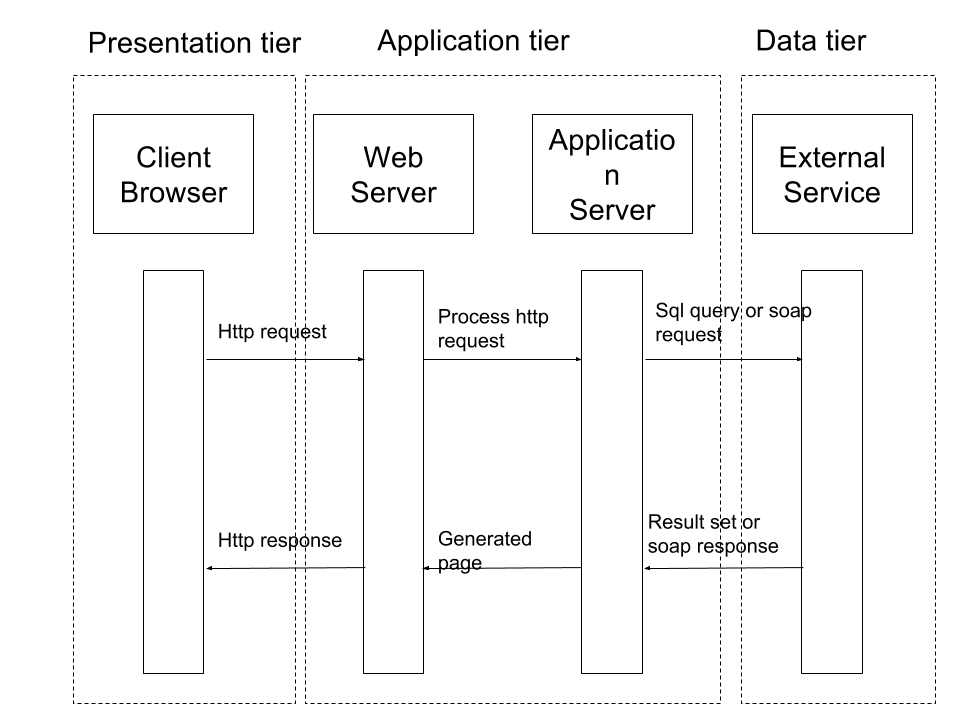
\includegraphics[width=0.75\textwidth]{client}
      	\caption{Web application structure}
      	\label{fig:pic1}
      \end{figure}
	  
    	Client-server structure helps to distribute application tasks or workloads
    	between the service providers called servers, and service requestors,
    	called clients. Client-server model helps to separate client and server logic, as
    	a result these parts can be independent and communicate via API. Client
    	server model grants several advantages:
    	\begin{itemize}
    	  \item Client and server parts can be developed separately.
    	  \item The application may have several clients.
    	  \item A client, for example a Web browser, can be already created.
    	\end{itemize}
    		
    	Client server model is closely related to a multi-tier architecture - the
    	concept where the parts of the system are divided into separate tiers. Web applications
    	 are often use three-tier architecture:
    	 \begin{itemize}
    	   \item Presentation tier is responsible for user interface generation and
    	   lightweight validation.
    	   \item Application tier (business logic tier) controls an application
    	   functionality, determines how data is created, displayed, stored and
    	   changed.
    	   \item Data tier - controls databases or other resources, provides access
    	   to the data.
    	 \end{itemize}
    	Multi-tier architecture allows any of the three tiers to be changed or
    	replaced independently, as a result developers have more freedom to use
    	external libraries and frameworks.
		
		All	applications have a lot of common features and problems which were already
		solved by developers beforehand. It is a good practise to take an already
		existing solution, than try to implement your own new one. That is why many
		modern applications are based on one or several software frameworks. In a
		rapidly changing and highly competitive business environment, choosing a right toolset is one of
		the key factors of the success.	 	
		
  \section{Vaadin}
  \label{ch:vaadin}
    Vaadin is a Java-based development framework for Web applications. ''Vaadin
    is designed to make creation and maintenance of high quality Web-based user interfaces easy.
   Vaadin supports two different programming models: server-side and client-side. 
   `` \cite[pr1.1]{bookVaaidn}
   \emph{Client-side} Vaadin code is executed in the Web browser as JavaScript
   code.
   \emph{Server-side} code is executed on the server as Java code on the Java
   Virtual machine(JVM).

   Client-side code is originally written in Java and then
   compiled to JavaScript using \emph{Vaadin Client Compiler}. Vaadin Client Compiler is based on Google
   Web Toolkt(GWT). The client-side code is responsible for rendering
   the user interface and send user interaction to the server. Vaadin allows
   developing client-side modules, which run in a browser without server
   communication. Client-side modules are used when there is no stable
   connection, for example mobile applications or  higly responsive UI logic is
   needed as in games. Client side module is compiled to Javascript and can be
   loaded to any web page.
   
   Vaadin Client Compiler has production and development modes. 
   In production mode Java  client-side code is compiled to one Javascript file. The script file in
   production mode is obfuscated, that is why reading or debugging it is nearly
   impossible. In production mode compilation should be called manually,
   after making changes to a client side Java code.
   In development mode client code is compiled at run-time, when Web page
   is reloaded. GWT links Java classes  with a compiled Javascript and gives
   an opportunity to debug code in a browser.
  
   Nowadays there are many standards and recommendations for Web
   developers published by World Wide Web Consortium (W3C) or  International
   Organization for Standardization (ISO), including recommendations for
   markup languages, Document Object Models (DOM) and standards
   for JavaScript. In spite of all the standards the difference between browsers
   and versions might be significant for the developer. The differences may vary
   from supporting different Cascading Style Sheets (CSS) tags
   and HTML5 features, differences in event handling and simply bugs. Vaadin
   client Compiler and GWT provide a wide browser support, eliminating the difference between browsers, and helping a
   developer to concentrate on essential parts of the application, instead of
   wasting time on cross-browser support. 
   
   Vaadin supports several popular Web browsers Internet Explorer 8 and newer
   versions, Firefox, Chrome, Safarin and Opera. Regression tests are run
   in all these browsers before every Vaadin framework release. Screenshot
   comparison as a part of regression testing see \ref{sec:screencompare},
   brings confidence to the developer that Vaadin components will not change
   their behaviour and appearance unexpectedly.
   
   A server-side code runs as a servlet in a Java Web server, serving HTTP
   requests. The servlet receives an HTTP requests from the client and
   interprets them as events for a particular user session.
   Events are associated with User Interface (UI) components and delivered to
   the event listeners defined in the application. After processing a request
   the servlet sends a HTTP response back to the client and the client renders
   the changes in UI received in the response.
   
   The communication between client and server sides is handled by a component
   connector. The main task of the connector is to send user interaction
   with the widget to the server-side and receive state changes from the server-side 
   and broadcast them to the widget see \ref{fig:vaadinClientCom}. 
    
	  \begin{figure}
      	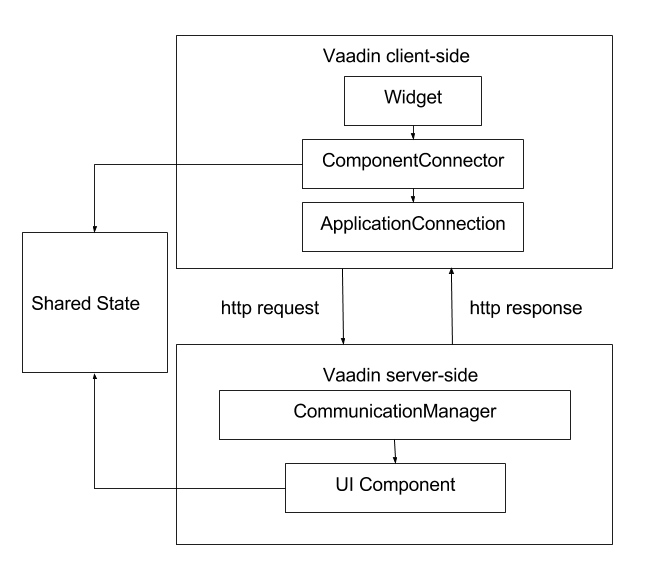
\includegraphics[width=0.75\textwidth]{vaadinClientCom}
      	\caption{Vaadin client server communication}
      	\label{fig:vaadinClientCom}
      \end{figure}
      
   For client to server communication connector uses Remote Procedure
   Calls(RPC) to the server-side. An RPC defines methods that can be called
   through the ``ServerRpc'' interface. After RPC is called from the client side
   it is serialized to a JavaScript Object Notation(JSON) and passed to the
   server side as a part of HTTP request. A server-side component registers an
   RCP handler which processes the RPC. 
   
   Server to client communication is done by using shared
   state. Shared state can be accessed both from client-side and server-side,
   but it is read-only on the client-side. When share state has changed it is
   serialized and send to the client side as a HTTP response. When state change
   occurs on the client side, the ``onStateChanged()'' method in the connector is called,
   allowing to change the connected widget.
   
   
  
   Vaadin framework handles all the client to server communication and provide
   a Java API for the user both for client and server sides. This positively
    influences the development process in the following way:
   \begin{itemize}
     \item The developer does not need to know several programming languages and one
    person may be involved in the developing of both a front-end and a back-end.
    This might be an important factor for small teams and speeds up the development
    process.
   \item Vaadin brings the power of Java into the Web development. Due to
    TIOBE index \cite{tiobeIndex} Java and C are the two most popular programming
    languages since 2002. This fact allows developer to use a great amount of
    already-made solutions such as building tools Maven \cite{maven} and Ant
    \cite{ant}, testing tools like JUnit \cite{junit}, frameworks for concurrent
    applications as Akka \cite{akka} \cite{akkaUseCases} and other libraries
    like Yodatime \cite{yodatime}, Guava \cite{guava} for different stages of development process.
  \end{itemize}  		
		
\section{Testing}
		Nowadays some companies still rely on manual testing or ignore this
		important part of software development. Such approach has several
		negative consequences:
		\begin{itemize}
			\item The developers are afraid of changing already written
			code. Because they do not have a confidence that their changes would not 
			break existing code. They stop cleaning their production code because they
			fear the changes would do more harm than good. ``Their production code begin
			to rot"
			\cite[p.123]{cleancode} 
			
			\item The effort of finding errors and	fixing them raises with the amount of
			code written, because the developers can not localize the place where the
			error is actual happening.
			\item Developing new features becomes harder, if they are based on the part
			of the system which have errors.
		
			\item Costs the whole system increases.
	 	 \end{itemize}
	 	 
	 	 To test easily the huge amount of code an automated testing is needed.	
	 	 Automated testing reduces the amount of work required to check Web applications as
	 	 well as Web sites, amplify software value, enhance reusability of test cases and improve time-to-market.
	   
		IEEE defines software testing as the process of evaluating a software
		system to verify that it satisfies specified requirements \cite{Xu1}. A set of
		requirements for a Web application includes security, performance,
		presentation, etc. We will focus on several requirements for the Web
		application which differ from desktop application. 
		
		One of the key factors which makes testing Web applications harder than
		testing desktop application is support of different browsers and operating systems and also
		different devices. Many desktop applications are developed to support some
		particular operating system or different versions of the product are developed
		and maintained for different operating systems. 
		
		Web applications on the	contrary should support not only different operating systems, but also
		different browsers and devices. So, if developers team decides to support
		three operating systems (Windows, OSX, Android), three type of devices (phone,
		tablet, PC) and three browsers (Chrome, Firefox, Internet Explorer) the number
		of possible variations is already 27. If you decide to support
		different version of browsers, which in some circumstances may vary a lot,
		the number of different configurations of tested machines will be close to
		one hundred. In this case manual testing is unexceptable, because it will lead
		to unwarranted expenses. 
		
		Another difference between Web and desktop applications is
		navigation on the Web page and between pages, the unexpected state change via
		the browser back button or direct Uniform Resource Locator(URL) entry in the
		browser. Some resources or parts of the application can be not
		accessible, due to connection problems or maintenance. Such unexpected
		behaviour may happen, and must be handled properly, not to crash the whole application.

    As mentioned previously one of the key factors for a successful
    development process is to pick a right toolset, this also applies to
    testing. In the chapter \ref{ch:Webtesting} we will present work done by
    other researchers and show how we can use it in creating a test framework
    for Vaadin applications.
      
\iffalse
		Web testing includes the different type of testing like:
		\begin{itemize}
		  \item functionality tests
		  \item compatibility tests
		  \item load tests
		  \item performance tests
		  \item integration tests
		\end{itemize}

		All these types of tests are equivalent important and picking a tool which
		will help to write these tests is not an easy task. 
		
		It is an advantage when	the testing tool is using same principles and similar programming language
		with other tools in the project. We think that using same programming language
		to write both tests and code is much easier for the developer. This idea is
		related to Test Driven Development(TDD), when tests are written
		before production code.
		
\fi				 
	\chapter{Web testing}
	\label{ch:Webtesting}

		There are several approaches for Web testing, the choice among them depends on
		different factors such as lifecycle of the project, technologies used, the
		budget, the professional level of developers. Two main ideas are Capture and
		Replay tests (C\&R) and programmable tests.
		
		\section{Capture and Replay}
		\label{sec:captureReplay}
			C\&R Web testing is based on capture/replay automated
			tools. \cite{CaptureReplay7} The software tester works with the Web
			application modeling user behaviour, the capture/replay tool records the
			whole session and generates the script, which can be executed later,
			repeating same actions without humans participation. Script editing might
			 be useful to adjust failed scripts accordingly
			to the changes of the Web page. Thought if the Web page was changed
			significantly, editing test script might be more expensive than recording the
			test from scratch. 
			
			We must admit that C\&R approach is very popular, there are plenty of
			frameworks both for desktop and Web applications such as TPTP GUI Recorder, SWTBot, QF-Test,
			Selenium IDE.
			The main advantage of this method of testing, is that the tester does not
			require to have experience in coding and building test cases with such tools is a simple task. 
			
			On the contrary, maintaining tests is harder and more expensive.
			The main problem is that editing generated scripts is harder than editing
			scripts written by a software developer. The test cases are strongly coupled
			with Web pages, contain hard-coded values. These factors lead to the
			problem, that very often the tester have to record a new test, instead of
			changing the existing ones. When using C\&R tools the tester can
			not use loose-coupling and decomposition, and other design techniques to make
			easy readable and maintainable tests. It is hard to use parts of already made
			test cases when creating new ones. Basically the main
			approach is to spend a lot of time recording tests all over again and again.
			Programmable tests can help to solve these problems.
			
		\section{Programmable tests} 
		\label{sec:programTests}
			Programmable tests are created by a tester manually. This method requires the
			person to have programming skills and takes more time, but programmable tests
			are more flexible and allow the developer to use bigger set of tools. The
			developer may use conditional statements to change execution of the test,
			loops to repeat same actions, exception handling, data structures like
			arrays, sets, trees, graphs, logging and etc. Programmable tests are more
			flexible and powerful than C\&R tehnique and provides the ability to create parameterized
			tests - tests which can be executed multiple times with different arguments.
			To show that programmable tests are more powerful than C\&R we provide an
			example.
			
			
			Suppose we have a Web framework with set of UI element classes and want to
			test that changing elements value triggers a value change listener event.
			First we create a Web page where we add elements we
			want to test (textfield, combobox, radio button, etc.) and an assertion input
			element. The assertion element will include a string, which will be
			compared with expected value.
			UI elements are added to a hash map as keys.
			Strings which will be set to the assertion element are added as values to the same map. Then we
			iterate through all values in the map and add elements to the Web page and
			set their ids. We also add value change listeners, which will set
			the value of the extra element according to the event triggered. Finally we
			get a Web page with set of elements. When setting value of an element with
			some id will set the assertion element to have the same id as value. For
			example if an element with an id ``textfield'' has changed its value the
			assertion element will have string ``textfield'' as value.
					
  \begin{lstlisting}
  public class TestWebPageClass {
  	static final String ASSERT_ELEM_ID="assertElementId";
  	 static Map<AbstractElement,String> map = new HashMap();
  	 static  {
    	   map.put(new TextField(),"textField");
    	   map.put(new ComboBox(), "combobox");
  	}
  
  	TextField assertionElement=new TextField();
  	public void createTestWebPage () {
  	    Iterator it = classToAssertValue.entrySet().iterator();
  	    while (it.hasNext()) {
  	    it.getKey().setId(it.getValue());
  	    addElementToWebPage(it.getKey());
  	    it.getKey().setValueChangeListener(event-> {
  	      assertionElement.setValue(it.getValue());
  	      });
  	  	}
  		addAssertElement();
  	}  
  	
  	public static <AbstractElement,String> getMap() {
  		return map;
  	}
  }
  \end{lstlisting}
      
      In our test we iterate through all elements in the map and find the
      element on the test Web page by id. Then set a value to this element,
      at this point the value change listener of the element should be triggered and set the value
      of the assertion element. In the last step we compare the value in the
      assertion element with a value in the map.
			
\begin{lstlisting}
public class ValueChangeListenerTestClass {
	<AbstractElement,String> map=TestWebPageClass.getMap();
	String assertElementId=TestWebPageClass.ASSERT_ELEM_ID;
	UIElement assertElement=findElementById(assertElementId);
       
    @Test
    public void testValueChangeListener() {
    	openWebPage();
        Iterator it = map.entrySet().iterator();
          
        while (it.hasNext()) {
        	Map.Entry pair = (Map.Entry)it.next();
        	UIElement elem=findElementById(map.getValue());
        	elem.setValue(``foo'');
        	String assertMessage=``Element with id=''+pair.getValue()
        	+ ``has wrong value'';
        
        	Assert.assertEquals(assertMessage,assertElement.getValue(),
        	pair.getValue);
        }
    }
}
\end{lstlisting}
  
      As mentioned before, the biggest advantage of programmable tests against
      C\&R is scalability. When using programmable tests, testing new elements
      requires just adding these elements to the map. But when using C\&R a
      tester should record same actions for each new element. If later for
      example we decide to have a test that checks that getValue() mehtod
      returns the same value as it was set with setValue method we can create
      a new test method which will use the same map of elements. 

\begin{lstlisting}
	//test getValue() and setValue()
	@Test
	public void testSetValue() {
    	openWebPage();
    	private String testValue="foo";
    	Iterator it = map.entrySet().iterator();
    	while (it.hasNext()) {
    		Map.Entry pair = (Map.Entry)it.next();
			UIElement elem=findElementById(map.getValue());
            elem.setValue(``foo'');  
            Assert.assertEquals(elem.getValue(),testValue);        
        }
    }
\end{lstlisting}

      As a result we can see that thought writing programmable tests with
      compare to C\&R is harder and requires more experience and skills, they
      provide more flexibility and scalability. The empirical study
       of developing tests for four different frameworks shows that the development of programmable tests is more time
      consuming (between 32\% and 112\%), but test maintanance requires less
      time (with a saving of 16\% and 51\%). As a result ``In general, programmable test cases are more
	expensive to write but easier to evolve than C\&R ones, with an advantage after
	two releases (in the median case)''.\cite{CaptureReplay7}

   \section {Other frameworks ideas}
   		Paper \cite{Xu1} and \cite{Zhongen2} describe of the capture-replay
   		tehnique.
   		The testing monitor agent chooses the user scenario (which is written by the tester/developer),
   		 then testing agent executes the scenario and outputs the testing
   		 resutls to the monitor agent. Then the monitor compares the test output
   		 with the expected result and prints the final report. The example of the
   		 test case in paper \cite{Zhongen2}
   		 \lstset{language=XML}
   		 \begin{lstlisting}
			 <request url = "http://mytestWebsite/login.asp"> 
			 	<parameter name = "name" value = "computer"/> 
			 	<parameter name = "password" value = "hello"/> 
			</request> 
			<response> 
			 	<match op = "contains" regexp=false select = 
			 	"/html/body" value = "Login Error!"/> 
			</response> 
   		\end{lstlisting}	
		This approach has one major disadvantage, such test framework can not test
		the application UI, it tests only server side logic, while client
		side stays untested. Another minor issue is that developer wants to write
		code and tests using same language, the reason is that code and tests are
		written in parallel, so testing framework should be very close to the
		developing framework and/or programming language.
		
		The paper \cite{testGen3} describes an improved tool for Web application testing. 
			``The test driver for testing the client-side pages has the structure as
			shown in Fig.1. (1)  is the parameter initialization part. This part reads the test data and 
		 initializes parameters shown in the  user interface form. (2) is the test 
		 execution part that executes the  user interface form on the target 
		 page. In the part (2), the control  script written in the script 
		 languages like Javascript simulates event user actions in the Web browser. (3) is the inner frame 
		 that contains the target page.'''
		  This tool allows to test client-side code, because the test driver
		  contains the target page and script to simulate user actions in the
		  Web browser. 
		  				Figure 1
		Both approaches 1 and 2 have one major disadvantage:
			Client side testing is not complete. Thought approach includes client side
			page, it does not provide any tool for testing appearence of the Webpage. The
			client side page may have bugs in css or html, for example if all html
			elements had css rule display:none, they would not be shown for user in the
			Web browser. Thought all user actions could be still emulated by javascript.
	\section {Challenges}
	\label {sec:challenges}
		Papers \cite{Xu1} \cite{Zhongen2} and \cite{testGen3} include very simple
		examples like login page. Real-life example may have dozens/hundreds of html
		elements on the Webpage see example of Gmail html page \ref{fig:gmailexample}.
		Web pages with big and branched DOM bring several challenges:
		\begin{enumerate}
		  \item Searching for required element may be very resource-consuming,
		  affecting time of the test execution. 
		  \item Changes in DOM may require changes in tests, which increase
		  application maintanance costs.
		\end{enumerate}
		
		\begin{figure}
		\label{fig:gmailexample}
		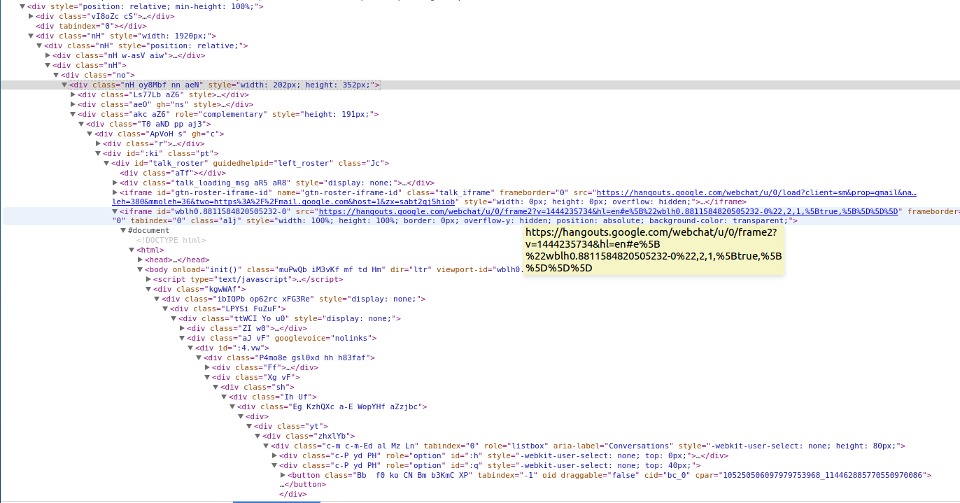
\includegraphics[width=0.75\textwidth]{gmail_example}
		\caption{Gmail DOM structure example}
		\end{figure}
		
		Testing frameworks allow several strategies for locating Web page elements:
		\begin{itemize}
		  \item By id -locates the Web page elements using their id values.
		  \item By name -locates the Web page elements using their name.
		  \item By tag - locates the Web page elements using their tag.
		  \item By class - locates the Web page elements using their class attribute.
		  \item By XPath - combines previous strategies and builds a search
		  path to an element in the DOM.
		\end{itemize}
		
		The choise between these strategies is a tradeoff between effeciency of the
		test and its complexity for developer. The research of Maurizio Leotta
		and Diego Clerissipaper in ``An Industrial Case Study about Web Page Element
		Localization" ``shows that ID-based methods for locating Web page elements are
		better than XPath methods''\cite{selenium4} showing that tests with search by
		Xpath executed more than three times longer than same tests with searching
		elements by Id. According to the same paper ID-based test require less
		maintenance effort, than the XPath-based test suites. In fact using searching by id for static HTML Web pages with small
		amound of elemnetn works well, but having dynamically generated HTML with 
		a lot of elements as in example \ref{fig:gmailexample} brings challengies.
		
		The biggest downside of searching by id strategy, is that every HTML element
		should have a unique ID. If the Web pages has a dynamically generated content,
		for example a table, where amount of rows depends on data, the
		developer has to add some logic to generate ID for each row and also verify
		that new ids do not conflict with already created ones. 
		
		In some circumstances the developer needs to get a set of elements by some
		criteria, for example get all elements with a specific tag or class selector
		and process them in a loop. 
		
		As we can see there is no one solution for searching elements on a Web page,
		which can be used in all cases. The developer should make a solution which
		searching algorithm to use based on requirements, but the testing framework
		should provide the developer different tools to choose from. In the next
		section we present Selenium - a software testing framework for Web
		applications, which allows to create C\&R \ref{sec:captureReplay} and 
        programmable tests \ref{sec:programTests}.Selenium  supports searching
        elements by id,tag, class, Xpath, etc and provides an opportunity to run tests in
        parallel.
		

 

\iffalse  
	\subsection{User interface testing}	
		Some information why user interface testing is important and also why
		automated user interface testing is even more important. So we are narrowing
		the scope of the problem, not to talk about all types of testing.

		
		Afterwards I will introduce Vaadin, what's the main idea behind the framework.
		Also here I will introduce Testbench tool and Selenium- the basis of
		testbench. Thought the testbench is already exists, I would like here to tell
		what are the reasons of having Testbench, why it is needed why it was started.
		What are pros and cons. Here I'm not talking in detail about Testbench, I'm
		just introducing it.
\fi


\chapter{Development of Testbench}
\label{ch:testbenchdevelop}
  
  The estimated time for developing Testbench4 was from two months to six weeks.
  Our team had four members:
  \begin{itemize}
    \item Anthony Guerreiro - developer.
    \item Dmitrii Rogozin - developer.
    \item Jonatan Kronqvist - tech lead.
    \item Mika Mutajarvi - developer.
    
  \end{itemize}
  
   This is a short period of time and to manage delivering a good-quality product you
    have to minimize overhead costs. We believe that a team should choose tools
    and methodology which suits its purposes. 
    Our team decided to use Scrum and Test Driven Development(TDD) for managing
    product development and try to be agile and flexible. 
    We decided to have two week sprints.

  \section{Scrum}
    Scrum is a management and control process that cuts through
    complexity to focus on building software that meets business needs. Management and teams are able to get their
    hands around the requirements and technologies, never let go, and deliver working software,
    incrementally and empirically. The Scrum Team consists of a Product Owner,
    the Development Team, and a Scrum Master.
    
  \textbf{Product Owner}(PO) - decides what features should the product have to
  maximally increase the satisfaction of the end user of the product and puts this features to the backlog.
  Backlog is a set of features in priority order.
  
  \textbf{Development team} - is
  a set of professionals that are working on implementing features of the product. 
  The team size should be from three to eight people. The team should work only on tasks from the backlog.
  
  \textbf{Scrum master} - a person who should help the team to increase their
  productivity by enhancing the understanding of teams strengths and weaknesses.

  The main idea of scrum is that development is done in short-time periods
  called sprints. Each spring consists of several phases:
  \begin{itemize}
    \item  Sprint planning - when team decides what tasks should be done during the
  sprint .
  \item   Main phase - when actual development is done.
  \item Sprint review - when team shows the results to the product owner.
  \item Retrospective - when team discuss what can be improved.
  \end{itemize}
 
  Sprint may take from one to four weeks. The development team should decide
  what sprint length suits their needs. During sprint planning the team chooses
  which tasks will be moved from a product backlog to a sprint backlog.
  One of the restrictions is that the task in sprint backlog should be done in one sprint.
  If the team thinks that the task can not be finished in one sprint this task
  should be divided into several subtasks. 
  
  Having such one-sprint tasks helps the scrum team to keep track of the
  progress easily and gives an opportunity to receive feedback for each
  completed task at the end of the sprint. This helps to detect problems at the early stages, when
  the errors does not have a tremendous feedback.
  Even if a feature was misunderstood by the development team
  and the team  has to redone it completely , the team wastes time equal to the
  length of the spring at maximum. While in a classical waterfall model,
   a sequential design process in which progress is seen as flowing steadily through 
   the phases of all development stages, 
  the error might be found much more lately, which will have a bigger negative impact.

  Another feature of Scrum is self organization of the team. The team should
  decide by itself which tool set to use. Tasks in scrum are not assigned to
  developers by a manager, but instead developers take items from the backlog by themselves.
  This approach saves time and reduces stress, because a person can pick a task,
  which he likes and understands. Developers pick tasks that they
  can finish before the end of the sprint.

  In our case we were not developing a new product, but releasing a new version.
  We did not find any arguments to change the tools were used in the previous
  release we describe them in section \ref{sec:toolsused} .

  \section{Test Driven Development}
  TDD is a very popular methodology of a software development. The main idea is
  to write tests first and then code. The main benefits of such approach are:
      \begin{itemize}
        \item The developer is sure that his code works as intended, because all
        his code is tested.
        \item The errors are found at early stage of the development cycle, which
        reduces the cost of fixing problems.
      \end{itemize}
      
      Three laws of TDD \cite[pp122]{Cleancode}[Book page 122]
        \begin{itemize}
          \item You may not write production code until you have written a failing unit test.
          \item You may not write more of a unit test than is sufficient to fail.
          \item You may not write more production code than is sufficient to pass the currently failing test.
        \end{itemize}
        
  \section {Tools used}
  \label{sec:toolsused}
  
  \subsection{Maven}
  Maven is a java-based software project management and comprehension tool.
  Maven is based around the central concept of a build life cycle. This means
  that the process for building and distributing a particular project(artifact) is clearly defined. There are three built-in lifecycles:
  default, clean and site. Users can define their own life cycle. 
  
  Life cycles  consist of phases.  The default life cycle includes the following phases:
  \begin{itemize}
    \item validate - validates the project is correct and all necessary
    information is available.
    \item compile - compiles the source code of the project.
    \item test - tests the compiled source code using a suitable unit testing
    framework. These tests should not require the code be packaged or deployed.
    \item package - takes the compiled code and packages it in its distributable
    format, such as JAR.
    \item integration-test - processes and deploys the package if necessary into
    an environment where integration tests can be run.
    \item verify - runs any checks to verify the package is valid and meets quality criteria
    \item install - installs the package into the local repository, for use as a
      dependency in other projects locally.
    \item  deploy - copies the final package to the remote repository for
    sharing with other developers and projects.
  \end{itemize}
  
  The life cycle phases are executed sequentially. For  example 
  running maven deploy executes all the  previous phases (validate, compile,
  test\ldots).
  
  All maven configurations are specified in the Project Object Model (POM) file.
  POM is an XML file that contains information about the project and configuration details used by Maven 
  to build the project. 

  Maven reduces the complexity of developing and maintaining big projects.
  Nowadays applications may depend on dozens of third-party libraries and
  frameworks. Managing those dependencies manually is very time consuming. Maven
  finds  and downloads the exact version of the library and adds it to the
  project.
  
   Maven profiles allow to have different configurations of your
  application for development and production or testing. All the maven
  configuration are in the same POM file, that is why editing and sharing
  configurations between members of the team is very easy. 

  Finally, you have a set of predefined configurations for your application
  for the whole team and any developer can checkout POM file from the repository
  call ``mvn deploy'' and he will have the same version of the application with all
  the specified parameters and downloaded dependencies. If you updated
  your dependencies or fixed an error, all your team members
  have to just checkout the new version of a POM file.
 
  \subsection{Trac}
  Trac is an enhanced wiki and issue tracking system for software development
  projects. Trac may include several projects. Users or developers can
  create tasks (also called tickets) for these projects. 
  
   Before development a new release a product owner goes through 
   the list of the tickets and add them to a new milestone.
  Milestone is a plan for the next release, which includes a set of tickets.

  Tickets have different value for the end user, but developers can not always
  assess that value by themselves. Product owner should help the development team
   to figure out the
  value of each ticket for the end user. Based on the value and time estimation
   each ticket should be prioritized.
  Prioritizing tickets is a very important task and should be done as soon as
  possible, preferable before coding starts. This gives a clear vision for all
  members of the team what should be done.

  In the Testbench4 project we used the Trac milestone as a product backlog. On
  the sprint planning we estimate which tasks can be completed at the end of the sprint 
  and move them to the sprint backlog. As a sprint backlog we used a scrum
  board.
  
  Scrum board is a white board, divided into several sections for example ``to be done'', ``in progress'', ``in review'',
  ``closed''. Paper stickers represent tickets and the person who is working on
  the ticket.  
  The workflow is the following - a developer picks the
  ticket from the sprint backlog queue called ``to be done'' 
  writes his name on the sticker and move it to the ``in progress'' section.
  After he submitted a patch to the code review he moves the sticker to another
  section and so on.
  
  Looking to the scrum board gives you a brief summary of every team member tasks and 
  also the current sprint progress. One can also find more detailed information
  about tickets and the project progress in Trac.
 
 \subsection{Git}
  As a version control system we used \textbf{Git} - distributed revision control system
  which focuses on speed, data integrity, and support for distributed,
  non-linear workflows. There are two types of revision control systems :
  
   \begin{itemize}
   \item Client-server - such version control systems as SVN and CVS, have a 
    a centralised model, where there's a copy of the current code on a central
    server, which users copy in order to work with locally. When a user makes
    some changes, he updates from the central version (in case other people have
    made changes in the meantime), solve conflicts (same part of code was
    changed by different people at the same time) that might have arisen, and
    then push their code back to the server. Afterwards other people can check
    it out again.

   \item Distributed revision control systems such as Git, are structured on a
    peer-to-peer basis: instead of one centralised repository. Every developer
    has their own repository and there is no main repository as in client-server
    control systems, all repositories are ``equal''. Though in practise developers
    create a ``master'' repository, where everyone push their own changes and pull
    changes made by other developers.
  \end{itemize}
  
  One of the biggest advantage of distributed systems is that repositories are
  synchronised by exchanging change-sets in the form of patches, in other words
  if you have changed two symbols, these two symbols plus some internal
  information - author, time, etc. On the contrary, in systems like SVN every
  time you pull changes from the central repository you are downloading 
  the whole snapshot of your application sources.
  
  Also Git lets developers to have their local history of changes and commits,
  but then when pushing changes to the master repository they can rebase these changes as one commit.
  This helps on one hand keep a local history of intermediate steps for
  developer, but on the other hand have only commits for completed changes
  or features in the main repository. 
  
  Git has a powerful set of tools including
  unix commands. For example to find all commits made by one person you can use
  log command and pipeline it to a pattern matching command like ``grep''.
  
   Git-blame command allows you to see the history of every line of your source
   code. If you have questions about some particular few lines of code,
   you can find an author of those lines and ask him a question.
   
   Git-bisect command - is a binary search against revision graph, which helps to find the commit which
   introduced a bug.

  \subsection{Teamcity}
  Teamcity - is a Web-based build management and continuous integration tool.
  Teamcity allows running multiple builds and tests under different platforms and environments.
  Teamcity build combines maven, ant builds, git command and bash scripts.
  
  Teamcity builds may be started automatically or manually. One option is to create a configuration 
  to run all  tests every night or to setup running tests on every git commit. Teamcity
  provides also build dependencies. If project A depends on a library B,
  Teamcity will first build library B with its dependencies and then start build
  project A.
  
  During the development cycle we used four different configurations.
  \begin{itemize}
  \item Running tests on every git commit. This configuration is started when
  Gerrit \ref{sec:gerrit} patch is submitted.
   Running all tests for all browsers is very time consuming and may take several hours. 
   That is why in this configuration includes only JUnit tests and PhantomJS
   tests, which does not need to run the actual browser.
   These tests show common errors for all browsers. Running those tests gives
    a developer a fast feedback, if his changes caused some problems.
   
   \item Running all tests on latest commit every night. This build triggers at
    specific time every night, when servers load is lower than during the day.
    This configuration includes all the heavy tests for specific browsers. All
    the tests are run on Google Chrome, Mozilla Firefox and Internet Explorer 8, 9, 10 and 11. 
    For every test suite Teamcity will run the specific browser on a test
    cluster. Running such tests is very resource consuming, but provides a
    confidence that the application is supported by all browsers.
    
    \item Snapshot build is run every night. This build publishes the latest
    version of the product to a maven repository.  Users can download
    the snapshot build with the latest version of the product, if they want to
    test new features, but do not want to wait for the release build.
    
    \item Release build is run when the team releases a new version of the
    product. This includes building all the dependencies, running all the tests,
    specifying the version of the product, creating release notes, making tag in
    the Git repository, publishing a new version to maven repository and Vaadin
    Web site.
   \end{itemize}

\subsection{Gerrit}
\label{sec:gerrit}
  Gerrit is a Web-based code collaboration tool. Gerrit allows developers to
  review patches made by other developers. Gerrit has a very easy system of evaluating patches:
  \begin{itemize}
  \item -2 (veto) - patch has major problems.
  \item -1 (disapprove) - patch has minor problems.
  \item +1 (approve) - no problems found.
  \item +2 (approve) - can be pushed to master.
  \end{itemize}
  
  The difference between +1 and +2 is that the patch can not be pushed to git
  repository without having +2. The reviewer can give +1 if he is not sure about his level of competence
  and want someone else to inspect the patch. 
  There are might be several configurations of the review process,
  figure \ref{fig:gerritTestbench} shows the process used in the
  Testbench4 project.

  Firstly, a developer submits his changes(patch) to Gerrit. Gerrit triggers the
  specific build in Teamcity. This build includes building the project and
  running tests. After this step is finished, Teamcity returns a report about the build,
  if there are problems the report is send to the developer and the patch is marked as -2. If all
  tests pass Gerrit marks the patch as ready for review and put it to the list
  of waiting for review patches.
  Afterwards the reviewer evaluates the patch. Given the patch -1 or -2 means
  that the developer should fix the problems, and submit the next version of the patch. 
  The process continues until someone  marks the patch as +2,
    meaning in can be pushed to git master repository.
    \begin{figure}
      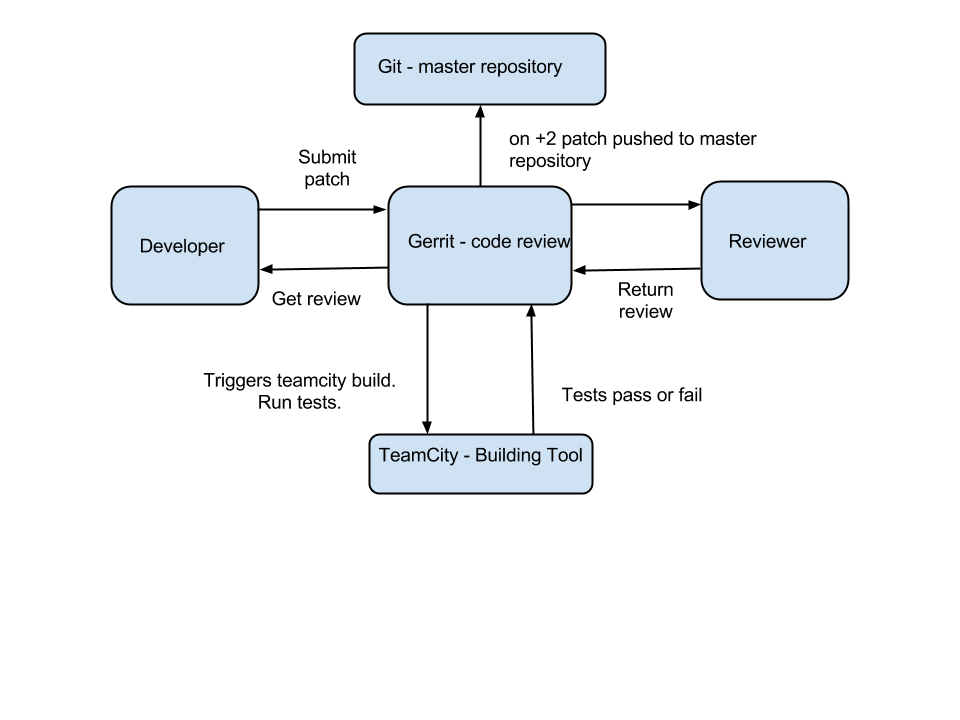
\includegraphics[width=0.75\textwidth]{gerrit1.png}
      \label{fig:gerritTestbench}
      \caption{Gerrit structure}
    \end{figure}
    
  Code review helps team members to follow similar code conventions, 
  keep code clean and readable and find bugs. Also code review helps developers to know more about 
  the whole project they are working in. Integrating Gerrit with an automated build tool, 
  such as TeamCity, allows to run tests before publishing commit for review. 
  The patch with failing tests is rejected automatically and an email with report
   for all failing tests sent to the author of the patch. 
   As an overall code review helps to keep source code quality on a higher level.

  \section{Testbench class diagram}

  The hierarchy of classes in Testbench consists of many tens of classes and each class has tens of methods.
  Here we will describe the most important classes and the basic principles see
  figure~\ref{fig:classdiagram}.
	\begin{figure}
		\label{fig:classdiagram}
	    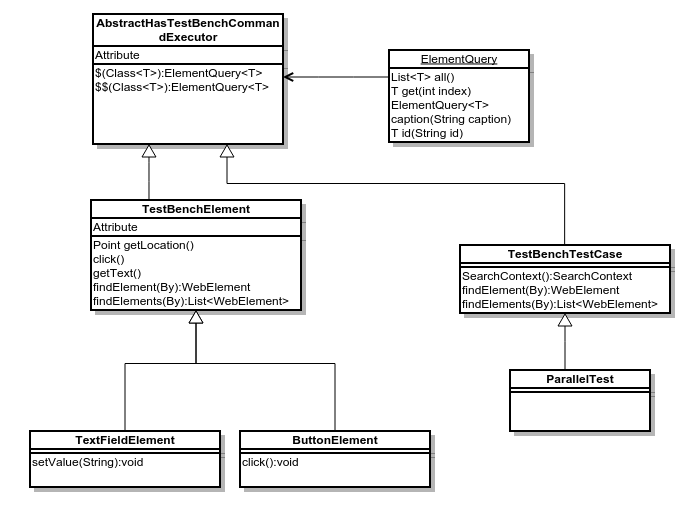
\includegraphics[width=0.75\textwidth] {umlDiagram.png}
	    \caption{Testbench class diagram}
    \end{figure}

\textbf{TestBenchCommandExecutor} handles client server communication
and provides screenshot comparison implementation.

\textbf{AbstractHasTestBenchCommandExecutor} class provides  `\$(Class clazz)'
and `\$\$(Class clazz)' methods which create a query for searching elements of
the given type.
 `\$' method builds a recursive search query and `\$\$' a non-recursive one.
 Non-recursive search query looks only for direct children of the element, while
 it is recursive analog looks through all children of the element. Children
 elements are inner HTML-elements. In example \ref{lst:domexample}
   button and check box input elements are children elements of the div element
   with id id1.
 \lstset{style=console}
  \begin{lstlisting} [caption=Simple DOM example,label={lst:domexample}]
  <div id="id1">
	  <input type="button">
      <input type ="checkbox">
  </div>
  \end{lstlisting}
  
  
\textbf{ElementQuery<T>} used for locating Web elements(Vaadin buttons, text
fields, labels, etc.) on the Web page. Generic parameter T specifies the type of a searched element. 
 ElementQuery class provides methods for searching the element based on
 element's id,class, caption or other criteria. These methods can be considered
 as filters in the query. ElementQuery uses the Builder pattern, 
 which helps to add several filters to build a specific query and after
 the query is built execute it.

Example \ref{lst:searchButtons} shows finding all children elements of the
parent element  which are buttons:
  \lstset{style=a1listing}
\begin{lstlisting} [caption=Search for all buttons,label={lst:searchButtons}]
AbstractHasTestBenchCommandExecutor elem = getParentElement();
List<Button> allButtons=elem.$(ButtonElement.class).all();
\end{lstlisting}
  
To restrict search for buttons with caption ``ok'' we add a caption filter to
the query see example \ref{lst:searchOkButtons}.
  \lstset{style=a1listing}
  \begin{lstlisting} [caption=Search for for button  with caption "ok", label={lst:searchOkButtons}]
AbstractHasTestBenchCommandExecutor elem =  getParentElement();
List<Button> allButtons=elem.$(ButtonElement.class)
	.caption("ok").all();
  \end{lstlisting}
  
\textbf{TestBenchElemenet} - is a base class for operating Vaadin components. It
includes methods to access properties common to all Vaadin elements,
such as "getSize()'', ``getLocation()'', ``getCssValue()'', etc.
TestbenchElement class uses Selenium WebElement class as a foundation and extend
it's functionality by using JavascriptExecutor,
which allows to execute JavaScript code, and change the default element behaviour.

\textbf{TestBenchTestCase} - an abstract super class of TestBench test.

\textbf{ParallelTest} - supports running test in parallel threads with several
browser configurations see \ref{sec:paralelTesting} for more details.

\textbf{ButtonElement, MenuBarElement, TableElement}, etc. - implement specific
Vaadin class features. The default naming conventions is Vaadin component name
plus ``Element''. In other words ButtonElement accesses buttons methods,
TableElement table methods and so on.

The important aspect is that hierarchy of testbench elements is similar to Vaadin elements.
That gives more flexibility when writing tests. The  developer/tester can
specify concrete class for getting access to specific methods of the element see example \ref{lst:specificExample}.
 
\lstset{style=a1listing}
\begin{lstlisting} [caption=Test for Vaadin table, label={lst:specificExample}]
  TableElement table= getElement();.$(TableElement.class).first();
  TableRowElement row=table.getRow(0);
 \end{lstlisting}
 
or use a more generic class to utilize method of a parent class, for example get
caption of all elements, see example \ref{lst:genericExample}.

\lstset{style=a1listing}
\begin{lstlisting} [caption=Caption test for Vaadin elements, label={lst:genericExample}]
List<TestBenchElement> elements=
	getElement().$(TestBenchElement.class).all();
List<String captions=new ArrayList<String ();
for(int i=0;i<elements.size();i++) {
	captions.add(elements.get(i).getCaption());
}
\end{lstlisting}

\section {Basic test case structure}
To use TestBench, the test case class should extend the TestBenchTestCase class,
which provides the WebDriver and ElementQuery APIs. A developer
can configure Testbench test by using following annotations:
\begin{itemize}
  \item @Rule -defines certain TestBench parameters.
  \item @Before - the annotated method is executed before each test.
  \item @Test - annotates the tested method.
  \item @After - the annotated method is executed after test.
\end{itemize}

A typical test case structure is the is the following:
\begin{itemize}
  \item Set TestBench parameters.
  \item Open the tested Web page URL.
  \item Find an element for interaction (Button, TextField).
  \item Interact with the elements (click buttons,menus,etc.).
  \item Find an element to check.
  \item Get and the value of the checked element.
  \item (optional) get screenshot.
\end{itemize}

A complete example of test UI class \ref{lst:appTestUI}  and a TestBench test
class \ref{lst:appTestClass} can be found in appendix A \ref{appendixA}.

\section {Results}
During Testbench4 development 41 tickets were closed the detailed information
about these tickets can be found in table \ref{table:tickets} in
appendix B \ref{appendixB}. 

To improve User Experience (UX) we have tried to reduce an amount of
configuration needed for using TestBench. We provide a complete working simple
test example as a part of build-in configuration.
Developers can use it as an example and extend it for their own requirements. Users may create a sample
Vaadin application via GUI using Vaadin Eclipse plugin or 
to create a sample Test via console Maven user should use a Vaadin Maven
archetype see \ref{lst:mavenexample}.
\lstset{style=console}
\begin{lstlisting}[caption=Create Vaadin sample application command.,label={lst:mavenexample}]
mvn archetype:generate 
	-DarchetypeGroupId=com.vaadin
	-DarchetypeArtifactId=vaadin-archetype-application
	-DarchetypeVersion=LATEST
\end{lstlisting}

After beta release we made several usability tests.
A Vaadin developer, without experience in using TestBench, manages to create and 
run a simple ``button-click'' test in less that 15 minutes. 

Vaadin Testbench 4 is released with Commercial Vaadin Add-On License 
(CVAL). But if you want to look results of our work and try it out you have two
options:

\begin{itemize}
  \item Free 30-days trial period.
  \item One year non-commercial license. All the details how to get it are at
  Vaadin blog \ref{vaadinBlog}.
\end{itemize}
\chapter{Testbench use}
\label{ch:testbenchuse}
In this chapter we will show several examples of using TestBench for writing
automated tests and show their value for different stakeholders. 

Originally TestBench was developed as a tool for writing acceptance tests for 
Vaadin framework it also used can be used to test any application written with
Vaadin. Acceptance test determines that requirements of a specification are met.
Currently (Fall 2015) there are over 6500 tests written for Vaadin framework.
All tests are running in Chrome, Firefox and Internet Explorer 9,10,11 during
night builds and before every release. New version of Vaadin framework can
not be released even with one test failing. This strict rule helps to keep
the quality of the product on a high level.

Having automated tests allow developers to refactor code without fear of
breaking previous work. Developers may not know all the details of the framework and make mistakes,
 failing tests give sufficient information about the problem 
 and give a confidence that new changes do not break existing code.
   
 Having automated acceptance testing is extremely important for large
 open-source projects, because this reduces a cost for developers to contribute
 to a project.  All patches to the framework are reviewed by Vaadin experts and
 running tests beforehand rejects fallible code.

 While automated tests have great value, there are circumstanceTs
 where a failing Testbench test gives a false alarm. One of the most fundamental
  problems of Web testing is that a developer can make a change that keeps
   the application completely correct, but breaks an automated test.   
That might be caused by changing DOM or CSS of the page, for example adding
an extra div may affect searching element by xPath. Such kind of problems 
occurs quite often when developing new features. Using ``screenshot on failure''
rule \ref{lst:screenshotOnFailue} helps to figure out such kind of problems. If
a developer get an error ``can not find an element on the Web page'', 
but this element is presented on a screenshot, most likely the problem is in
locating the element code.

Especially in agile development when work is done in small iterations/cycles, 
changes in code require changes in testing. This gives a fast feedback and
 an opportunity to find and fix problems early, but also brings frustration
for developers that they have to fix problems both in code and tests. 
That might bring a false attitude that writing tests on early stages of the project,
 when there is no clear picture of the final product,
 increases the amount of work for developers. 
 
 We are sure that writing tests reduces an overall work,
 even if these tests have to be changed often.
 Usually a good rule is that every patch should add or edit at least one test suite, that
 also ease the reviewers job, because a test suite explains what is the reason of the patch. 

In addition to having value throughout the development life cycle,
Testbench tests are valuable artifacts to get end-users feedback.
Because Testbench tests are executed in a browser, tests can be used 
for demonstrating framework or application features to the end-user. 
  
To demonstrate the usage of Testbench we will create a test for a Vaadin table
component extension. Developing Vaadin components is outside the scope of
this work, we assume someone extended a Table component by adding a filter field to
it. Typing value in the filter field filters values of the underlying table see
figure \ref{fig:filtertable}.
	\begin{figure}
	\centering
	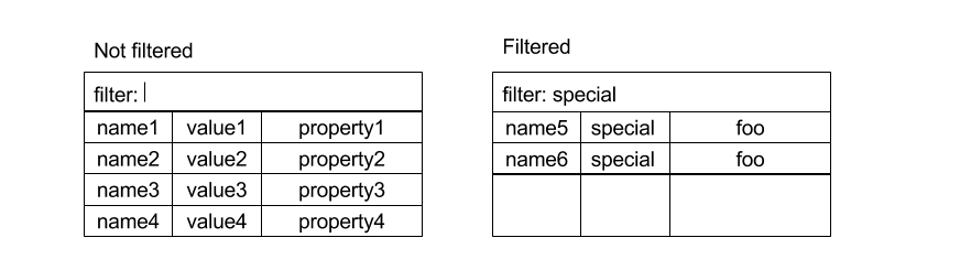
\includegraphics[width=0.75\textwidth]{filtertable}
	\caption{Table component extension example.}
	\label{fig:filtertable}
	\end{figure}

An essential  part of a Test for the filter feature is represented in listing
\ref{lst:testbenchTest}. 

 \lstset{style=a1listing}
  \begin{lstlisting} [caption=Example of table test,label={lst:testbenchTest}]
TableElement table = getTableElement();
TextFieldElement filterElement=table.
	$(TextFieldElement.class).id("filter-field").first();
filterElement.setValue("special");

//Comparing filtered values
TableRowElement row=table.getRow(1);
assertEquals(row.getCell(0).getValue(),"special");
  \end{lstlisting}

In the next section we will show how to improve this test by using
Behaviour-Driven Development(BDD) framework.

\section{Integrating with Behaviour-Driven Development frameworks}

The main goal of BDD is to get executable specifications of a system.
In other words BDD frameworks allow  to write user-stories in
common language, for example English, and associate them with automated
acceptance tests.

Testbench can be integrated with such BDD frameworks as JBehave or Cucumber.
Tests in JBehave are called scenarios see example of JBehave scenario
\ref{lst:scenario}.

 \lstset{style=console}
  \begin{lstlisting} [caption=JBehave scenario,label={lst:scenario}]
Scenario: filter table contents
Given web-page with table
When typing special to filter field
Then value in row 1 and cell 0 is special
  \end{lstlisting}
User story steps are matched into actual Java tests using annotations. 
The method with an annotation interact with an application and perform the actions needed.
Since TestBench tests are pure Java code and BDD steps can be run as JUnit tests, we can combine these to make
JBehave run TestBench tests.

We start by extending the TestBenchTestCase  and use JBehave's ``\@BeforeScenario''
annotation to open a tested Web page.  @Given @When and @Then annotations are
linked with corresponding steps in the user scenario.
To pass parameters from the user-scenario step to a Java method "\$"- special symbol is used.
JBehave implicitly casts passed value to a parameters type. The complete example
of the test is in appendix A \ref{lst:testbenchTest}.

To link a Java class and a textual story file we need to create a configuration class.
The simplest configuration is a one-to-one mapping between a Java class and a textual story file
see example in appendix A \ref{lst:jbehaveConfig}. 

So we can have both a user-story for our test explaining what should be done and a browser executed
test showing the actual implementation. Picture with user story and browser implementation. We believe that user-stories 
scenarios greatly ease communication between stakeholders, 
especially if some of them do not have relevant technical background.
So user-stories can be shared between stakeholders to show what is done and what
is planning to be done, if there are questions 
executing these user-stories in a browser will help to reveal more details about it. 
   

 %   Here I would describe how Testbench is used in Vaadin. How many tests are
    % in Vaadin. How we run them, how failed tests are fixed what are the problems
 %   and benefits. What features of the Testbench are used (parallel testing
 %   run, searching elements on web-page by id,name,class, xpath, etc.)
    
 %   Then I would like to mentioned how user/developer may use Testbench, what
    % is needed. Unfortunatelly it's really hard to find data to meausure the profit
 %   of using testging tools. It would be really nice to have a big project and
 %   have development with/without testing and see the end result, but I think
 %   it's really unlikely to happen. But may be there were some similiar
    % studies, at least for other tools.
   	
  

\iffalse
 \subsection {Comparing Testbench with other tools}
    Here I will compare testbench to some other testing tools for example
    Selenium, what are benefits of using Testbench. The main idea is to focus
    that Vaadin is a client-server framework, so all Vaadin components have
    client and server side code, and it's important to test both. I want to show
    what problems may happen if using only Selenium and test only client side
    code, so that server side isn't tested. 
    
    Also I would like to compare how complicated is to right Selenium and
    Testbench tests. How much code is needed to test button click for example,
    or sending text to a textField.
    
    Compare speed of running tests. In Vaadin we run tests every night, and
    sometimes it takes too much time, so I would like to mention ,what are the
    problems/challenges in having a lot of tests.

      
 \subsection {Vaadin integration}
    Testbench using some features of Vaadin framework, for example searching
    elements by vaadin selectors. So I want to describe how integration with
    Vaadin is done. What are the challenges. For example what would happen when
    using different versions of Testbench with different versions of Vaadin.
\fi    

 \section {Discussion and Conclussion}
 	Middle of April/ End of April
 	\subsection {Summary}
 	  What has been done. What were the challenges how they were solved.
 	\subsection {Advantages and disadvantages}
 	\subsection {Future work}
 	
 	
	\begin{thebibliography}{7}
	
		\bibitem{Xu1}
			Lei Xu, Baowen Xu,
			"A framework for Web applications testing.",
			Proceedings of the International Conference on Cyberworlds.2004, pp.300-305
		\bibitem{Zhongen2}
		Qian Zhongsheng,Miao HuaiKou,Zeng Hongwei.
		 A practicalweb testing model for web application testing[C] .
		 Third International IEEE Conference on Signal-Image Technologies and
		 In-ternet-Based System. 2007, pp.434-441.
		 
		\bibitem{Cleancode}
		Robert C. Martin,
		Clean Code: A Handbook of Agile Software Craftsmanship,
		Prentice Hall PTR, Upper Saddle River, NJ, 2008
		
		\bibitem{testGen3}
		Seung Hak Kuk, Hyeon Soo Kim,			
		"Automatic Generation of Testing Environments for Web Applications.",
		Computer Science and Software Engineering, 2008 International Conference on
		(Volume:2 ). 12-14 Dec. 2008, :694 - 697
		
		\bibitem {selenium4}
		M. Leotta, D. Clerissi, F. Ricca, C. Spadaro,
		"Repairing Selenium Test Cases:An Industrial Case Study about Web Page
		 Element Localization," in the Proc. of Sixth International Conference on Software Testing, Verification and Validation, pp. 487-488, 2013. 
		\bibitem{pageObject5}
		M. Leotta, D. Clerissi, F. Ricca, and C. Spadaro. Improving test suites
		maintainability with the page object pattern: an industrial case study.
		In Proceedings of the 6th International Conference on Software Testing, Verification and Validation Workshops,
		ICSTW 2013, pages 108-113. IEEE, 2013. 
		\bibitem{CaptureReplay7}
		
		
		\bibitem{performance6}
		Angmo R. , Sharma M.	
		Performance evaluation of web based automation testing tools.,
		Confluence The Next Generation Information Technology Summit (Confluence),
		2014 5th International Conference. 25-26 Sept. 2014, pp. 731 - 735
		\bibitem{webAppTesting8}
		Sebastian Elbaum, Gregg Rothermel
		Leveraging User-Session Data to Support Web Application Testing
		\bibitem {bookVaaidn} 
		 Author name.
		\bibitem {tiobeIndex}
		http://www.tiobe.com/index.php/content/paperinfo/tpci/index.html
		\bibitem{vaadinTestbenchSite}
		https://vaadin.com/add-ons/testbench
		\bibitem {maven}
		http://maven.apache.org
		\bibitem {ant}
		http://ant.apache.org
		\bibitem {junit}
		http://junit.org/
		\bibitem {yodatime}
		http://www.joda.org/joda-time/
		\bibitem {guava}
		https://github.com/google/guava
		\bibitem {akka}
		http://akka.io/
		\bibitem {akkaUseCases}
		http://doc.akka.io/docs/akka/snapshot/intro/use-cases.html
		\bibitem {vaadinAkka}
		https://github.com/rogozinds/VaadinWithAkka
	\end{thebibliography}
  \section {Appendix}
\end{document}

//TODO
{Other frameworks ideas} part give a name to all aprroaches or at least a link
add picture of the framework tool